%!TEX root = ../physical-olympics-2.tex
\chapter{万有引力}


\section{有心力下质点运动}

天体运动中起到核心作用的相互作用力都是\emph{有心力}(central force),\,事实上不光是天体运动,\,任意两个可以近似为质点的物体之间的相互作用力,\,根据牛顿第三定律的要求,\,其受力方向都必须沿着两个物体的连线方向.\,那么我们只要做两个要求,\,这就构成了一个有心力问题:

一是,\,这个力必须是保守力,\,即,\,它必须由势能生成:
\[V(\bs{r}_1,\,\bs{r}_2):\quad\,\bs{F}_1=-\nabla_1V\;,\,; \bs{F}_2=-\nabla_2V\]

根据我们之前的说法,\,根据对称性或牛顿第三定律,\,这个势能其实就是两个质点连线距离$R$的函数$V(R)$.\,而以$1$为中心向$2$引$\bs{R}$矢量,\,则:
\[\bs{F}_2=-V'(R)\bs{e}_{\bs{R}}=F(R)\bs{e}_{\bs{R}}\]

二是,\,中心物体$1$必须不动或者是近似不动.\, $1$不动是指有外力作用在$1$上以维持其静止.\,但$2$上不应该有这样的外力,\,而仅仅是在$1$对$2$产生的$\bs{F}_2$作用下做运动.\,$1$近似不动是比如考虑太阳系这种典型情况,\,太阳虽然受到多个行星对它的万有引力,\,但是由于自己质量过重从而近似是不动的.\,即使是地球月亮构成的二体问题,\,地球和月亮并不一定能认为都不动,\,我们也有相应的转化为有心力问题的方法,\,见后.\,最后当然,\,也有一些更简单的情况,\,$2$受到一些更复杂的体系对它的力构成了有心力$F(R)$,\,比如弹性绳对绳端质点的拉力.

在有心力场中运动的物体,\,其基本的牛顿定律可以写作:
\[m\ddot{\bs{r}}=F(r)\bs{e}_r\]

可以把这个方程作为一切讨论的起点.\,或者进一步,\,我们先发现:

\subsection{运动的一般特征}

首先,\,有心力场中运动的质点必然在一个平面上运动.\,这一点既可以通过初始条件判断$\bs{r}_0$和$\bs{v}_0$的平面就是运动平面.\,也可以通过下面的角动量守恒来发现这一点.\,正是这样,\,在运动平面上建议极坐标是方便的,\,用极坐标写出的牛顿定律分量式为:
\[\left\{\begin{array}{rcl} m(\ddot{r}-\dot{\theta}^2r) &=& F(r)\\ m(\ddot{\theta} r-2\dot{\theta}\dot{r})&=& 0\end{array}\right.\]

除了牛顿定律以外,\,还有两个可以变通使用的结论:\,角动量和能量都是守恒的:

角动量守恒的原因是有心力对力心没有力矩.\,角动量的方向垂直于运动平面.\,极坐标下大小写为:
\[L=m\dot{\theta}r^2={\rm Const.}\]

而习惯上通常把质量$m$省略后的量单独提出来,\,它实际上是面积速度的两倍:
\[\dot{\theta}r^2=h=2\frac{\ud A}{\ud t}\]

也就说,\,面积速度不变是有心力问题的普遍特征,\,这也是开普勒第二定律的一种推广形式.

第二个守恒量是哈密顿量:
\[H=\frac{1}{2}m(\dot{r}^2+\dot{\theta}^2r^2)+V(r)={\rm Const.}\]

守恒到的值直接叫做能量$E$.\,通常我们喜欢把这个式子移项写作:
\[\dot{r}^2+\dot{\theta}^2r^2=\frac{2[E-V(r)]}{m}\]

\subsection{有心力问题的求解}

有心力问题的求解可以指一定初始条件下,\,轨迹方程$r(\theta)$的求解.\,也可能需要进一步求出运动方程$r(t)$和$\theta(t)$的具体形式来.\,通常还有两种常见的提法:

\begin{wrapfigure}[14]{o}[-10pt]{6cm}
\centering
\vspace{-0.5cm}
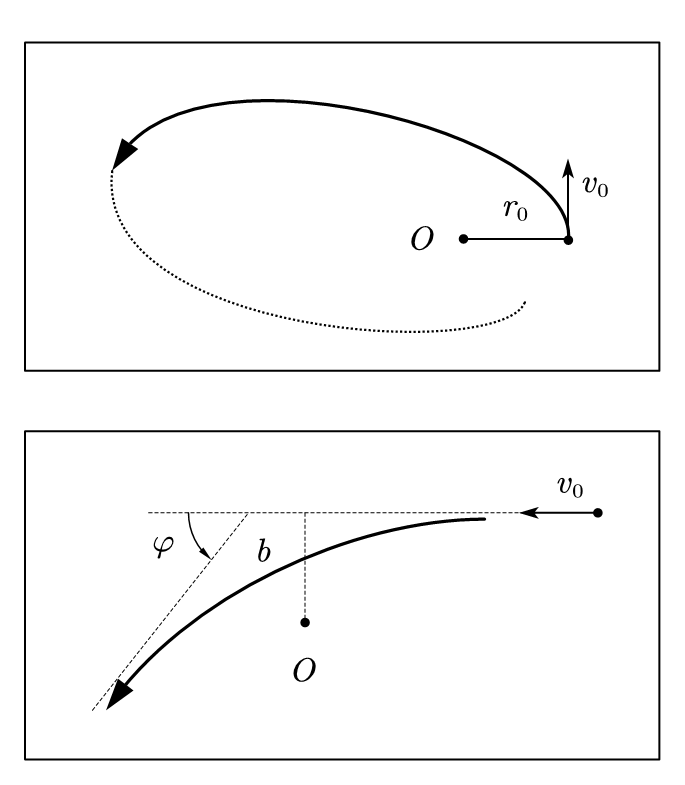
\includegraphics[width=6cm]{image/6-5-1.png}
\caption{定态问题与散射问题}
\end{wrapfigure}
一是\emph{定态问题}(stationary state problem)的求解:\,例如直接从距离力心$r_0$给一个垂直半径方向的速度$v_0$.\,求解之后的运动.\,不难理解,\,只有\emph{引力}(attraction)才能形成束缚的态,\,\emph{斥力}(repulsion)就不行.\,而要想这个态在动力学上是``稳定''的,\,后面就知道还需要这个力符合一定的条件.\,这一个问题在微观上也存在对应的量子力学版本.

二是\emph{散射问题}(scattering problem)的求解:\,粒子从无穷远出发以一定的初速度$v_0$和\emph{瞄准距离}(impact parameter)$b$入射,\,经过一个有心力影响后轨迹发生偏移.\,求解过程中,\,尤其是散射末态的粒子状态.\,由于轨迹必然存在对称性,\,出射过程基本上就是入射过程在另一个角度处的时间反演.\,所以经典物理中关注的量主要是散射角$\varphi$的大小,\,它被定义为散射前后运动方向的夹角.\,不难看出,\,不管是引力还是斥力都会造成散射.\,但是散射问题对有心力也存在一个要求,\,它在无穷远处必然对粒子没有影响,\,即,\,不管是势能还是力都要衰减到零.\,这个要求实际上叫做\emph{短程力}(short-ranged force).\,但它的严格定义和个别性质也需要上升到量子力学的散射问题才能解释清楚.\,比如万有引力其实就不属于短程力而是\emph{长程力}(long-ranged force),\,而超过平方的幂次反比力都是短程的.\,尽管前者的散射问题也经常被拿来讨论.\,散射问题不仅存在量子力学版本,\,引力场下的光线偏转问题也是一个非常经典的广义相对论问题.\

而目前求解经典的有心力问题通常有两种思路:

\vspace{0.5cm}

{\heiti 1.\,有效势能法}

\vspace{0.2cm}


利用两个守恒量,\,实际上就等于把原来的二阶微分方程求解的问题转化为了一阶微分方程的问题.\,然后再利用角动量守恒式子把$\dot{\theta}$用$r$来表示并代入能量守恒.\,我们得到:
\[\frac{1}{2}m\dot{r}^2=E-V(r)-\frac{mh^2}{2r^2}=E-V_{\rm eff}(r)\]

第一点是,\,问题立马变成了一个一维动力学问题.\,第二点是,\,这个问题等价于一个粒子$m$在一维势能场$V_{\rm eff}(r)$中做运动的问题.\,正是因为这个原因,\,我们把$V_{\rm eff}(r)$称作有心力问题的\emph{有效势能}(effective potential):
\[V_{\rm eff}(r)=V(r)+\frac{mh^2}{2r^2}\]

利用这种方法,\,物理意义上最显著的一点就是可以方便我们考察定态的存在性和动力学稳定性.\,显然,\,在一维运动中,\,仅有当在$r\in(0,\,+\infty)$下存在``山谷'',\,即一阶导数等于零,\,二阶导数大于零的点才有可能造成稳定的振动,\,它就是我们要寻找的束缚态.\,而这一点强列依赖于势能的具体形式.\,考察引入的``离心势能''项的导数,\,我们发现:
\[V_{\rm cf}=+\frac{mh^2}{2r^2}\quad \Rightarrow\quad V_{\rm cf}'=-\frac{mh^2}{r^3}\;,\;V_{\rm cf}''=+\frac{3mh^2}{r^4}\]

故这是一个倾向于往外推质点的力,\,而本身具有让质点稳定的因素.\,那么为了使得存在$V_{\rm eff}'=0$和$V_{\rm eff}''>0$的点,\,就要求$V'>0$必然成立,\,即必须是引力.\,且$V''$虽然可以小于零但不能太小.

我们考察幂次的引力$F=-kr^n$,\,那么它对应的势能为\footnote{$n=-1$时,\,$V=k\ln r$}:
\[V=\frac{kr^{n+1}}{n+1}(n\neq -1)\quad ,\quad V'=kr^n \quad ,\quad V''=nkr^{n-1}\]

结合平衡条件可以发现存在平衡点:
\[V'+V_{\rm cf}'=0\quad\Rightarrow \quad R=\left(\frac{mh^2}{k}\right)^{\frac{1}{n+3}}\]

那么在这个点处的稳定性就取决于二阶导数:
\[V''|_{r=R}=\frac{mh^2}{R^4}\left(3+n\right)\]

由于除非$h=0$,\,即纯径向运动,\,系数必然是大于零的.\,故分为两类情况:
\begin{figure}[H]
\centering
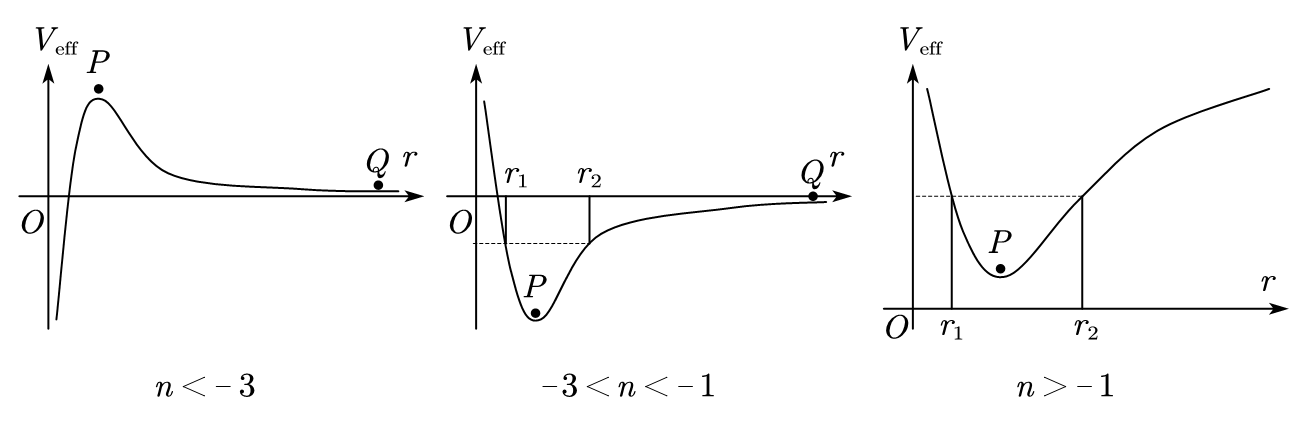
\includegraphics[width=16cm]{image/6-5-2.png}
\caption{三类幂律力}\label{6-5-2}
\end{figure}


一是,\,$n\leq -3$,\,即超过三次以上反比的力场,\,这样的力场不可能造成稳定的动力学运动.\,其势能函数图像如图\ref{6-5-2}左.\,平衡是可以造成的,\,此时径向上始终保持$r=R$,\,即停留在图中的$P$点.\,角向上$\dot{\theta}=h/R^2$,\,其实就是在做匀速圆周运动.\,但是这个圆周运动动力学不稳定,\,一旦存在径向上微扰,\,要么轨道无限向力心坍缩,\,要么向无穷远转移而失去力心的束缚.\,$n=-3$的特殊情况值得引起关注.\,此时,\,如果$h=\sqrt{k/m}$,\,那么势能恒等于零,\,对应大量不稳定的匀速圆周运动.\,而如果$h>\sqrt{k/m}$或$h<\sqrt{k/m}$,\,两者势能都是单调的不存在束缚态的可能性,\,前者会无限远离力心后者将无限接近力心.\,总之,\,$n<-3$都是不稳定的情况.

二是,\,$n>-3$下的所有力场都是稳定的.\,也就包括常见的平方反比力场.\,图\ref{6-5-2}的中,\,右图都是这种情况.\,$P$点具有稳定性.\,从而束缚态其实就是指在$P$点左右的振动和对应的角向运动的合成.

对束缚态和散射态的求解能给出哪些共同的结论?\,首先让我们计算束缚态下$r_1$到$r_2$间振动的周期,\,也就是径向运动的动力学周期.\,这个问题和$r(t)$的求解方法是共同的.\,只需要对之前的能量守恒式移项后积分:
\[\dot{r}=\sqrt{\frac{2[E-V(r)]}{m}-\frac{h^2}{r^2}}\]
\[T=2\int_{r_1}^{r_2}\frac{\ud r}{\sqrt{\frac{2[E-V(r)]}{m}-\frac{h^2}{r^2}}}\]

其中$r_1$为过程中最靠近力心的点,\,通称\emph{近心点}(pericenter),\,而$r_2$则为\emph{远心点}(apocenter).\,它们都是以上积分分母恰好为零的点,\,使得该积分成为一个标准的瑕积分.\,在$r_2$不是无穷大的情况下,\,该积分总是有限的.

我们还可以计算在近心点和远心点运动过程中质点转过的角度.\,这一点只需要找到角度的导数:
\[\dot{\theta}=\frac{h}{r^2}\]

并与之前的半径导数来做比:
\[\frac{\ud \theta}{\ud r}=\frac{h}{r^2\sqrt{\frac{2[E-V(r)]}{m}-\frac{h^2}{r^2}}}\]

这就能得到角度:
\[\Delta \theta =\int_{r_1}^{r_2}\frac{h\ud r}{r^2\sqrt{\frac{2[E-V(r)]}{m}-\frac{h^2}{r^2}}}\]

最后考虑散射问题的普遍结论.\,首先,\,幂律形式的力显然如果$n\geq-1$,\,这样的力对应的势能在无穷远处并不是$0$.\,将造成无穷远处具有一定初动能的物体来到近处时具有无穷大动能的发散问题.\,故我们讨论的范围局限在$n<-1$的幂律力,\,引力斥力皆可.\,十分类似地,\,如果计算从无穷远来到无穷远去发生的位矢的转角,\,为:
\[\Delta \theta =2\int_{r_1}^{\infty}\frac{h\ud r}{r^2\sqrt{\frac{2[E-V(r)]}{m}-\frac{h^2}{r^2}}}\]

再进一步注意到由初始条件确定的的守恒量各为:
\[h=v_0b\quad;\quad E=\frac{1}{2}mv_0^2\]

代入化简,\,我们要计算的偏转角$\varphi=\pi-\Delta\theta$就成为了:
\[\varphi=\pi-2\int_{r_1}^\infty \frac{v_0b\ud r}{r\sqrt{v_0^2(r^2-b^2)-2r^2V/m}}\]

当$n\geq-1$时偏转角的积分不会存在发散的问题.\,永远是一个有限值.

\vspace{0.5cm}

{\heiti 2.\,比耐方程法}

\vspace{0.2cm}

另一种思路执着于求解二阶形式的方程,\,但是通过变形转化为轨迹方程.\,具体来说,\,半径的一阶导数被我们化为:
\[\dot{r}=\frac{\ud r}{\ud \theta}\cdot\frac{\ud \theta}{\ud t}=\frac{h}{r^2}\cdot \frac{\ud r}{\ud \theta}\]

而二阶导数就能继续化为:
\[\ddot{r}=\frac{\ud }{\ud \theta}\left(\dot{r}\right)\cdot\frac{\ud \theta}{\ud t}=\frac{h}{r^2}\cdot\frac{\ud }{\ud \theta}\left(\frac{h}{r^2}\cdot \frac{\ud r}{\ud \theta}\right)=\frac{h^2}{r^4}\frac{\ud^2 r}{\ud \theta^2}-\frac{2h^2}{r^5}\left(\frac{\ud r}{\ud \theta}\right)^2\]

这样还不足以使得问题简化.\,因为如果代入径向的牛顿定律,\,得到的结果:
\[\frac{\ud^2 r}{\ud \theta^2}-r-\frac{2}{r}\left(\frac{\ud r}{\ud \theta}\right)^2=\frac{r^4F(r)}{mh^2}\]

还不见得是一个如何简单的方程.\,\emph{比耐方程}(Binet equation)的不平凡之处在于它对半径进行了反演.\,就是考虑一个倒数变换:
\[u=\frac{1}{r}\]

它可以把之前的运动轨迹的内侧翻到外侧去.\,那么如果依然保持$\theta$自变量不变,\,轨迹的新导数为:
\[r=\frac{1}{u}\quad,\quad \frac{\ud r}{\ud \theta}=-\frac{1}{u^2}\frac{\ud u}{\ud \theta}\quad,\quad \frac{\ud^2 r}{\ud \theta^2}=-\frac{1}{u^2}\frac{\ud^2 u}{\ud \theta^2}+\frac{2}{u^3}\left(\frac{\ud u}{\ud \theta}\right)^2\]

代入之前的轨迹微分方程,\,发现方程简单地变成了:
\[\frac{\ud^2 u}{\ud \theta^2}+u=-\frac{F(\frac{1}{u})}{mh^2u^2}\]

这个简单的方程就可以帮我们快速解决一部分有心力问题的基础轨迹.

\section{万有引力下天体运动}

万有引力即以下\emph{平方反比力}(inverse-square force):
\[F(r)=-\frac{GMm}{r^2}\]

任何平方反比力下的运动性质都是类似的.\,我们以引力为正.\,事实上经典物理喜欢用$k^2=GM$来指称中心力心产生力场的强度,\,称作\emph{高斯常数}(Gauss constant).\,我们这里用$k=GM$来表示引力的强度.\,这样$k<0$就表示斥力.\,而其它平方反比力,\,比如库仑力也就归为同一种:
\[F(r)=\frac{Qq}{4\pi \varepsilon_0 r^2}=-\frac{km}{r^2}\quad\Rightarrow \quad k=-\frac{Qq}{4\pi\varepsilon_0 m}\]

于是,\,在平方反比有心力下质点的运动问题,\,就构成了经典力学历史上第一个用来解决的里程碑式的大问题,\,它和它后来的各种变式,\,统称为\emph{开普勒问题}(Kepler problem).

为了以最快速度得到它的解,\,我们直接使用比耐方程,\,将力的函数用$u$表示并代入:
\[\frac{\ud^2 u}{\ud \theta^2}+u=\frac{k}{h^2}\]

这就已经得到它的解了,\,在合适的极坐标初始角度下写作:
\[u=\frac{k}{h^2}(1+e\cos\theta)\]

其中$e$是根据初始条件确定的常数.\,再倒过来便是:
\[r=\frac{h^2/k}{1+e\cos\theta}=\frac{p}{1+e\cos\theta}\]

不管$e$,\,$p$的正负和取值情况,\,这都表示一条圆锥曲线方程.\,可能是椭圆,\,抛物线,\,双曲线三者之一.\,我们还因此得到了一个恒等式$p=h^2/k$.

\vspace{1cm}

比耐方程固然简单.\,但是它对我们解决一个天体运动的含初始条件的具体问题帮助不大.\,为了得到一种行之有效的方法,\,我们重新回到有效势能的方法.\,现在我们代入势能函数:
\[V=-\frac{km}{r}\]

得到用$\dot{r}$和$\dot{\theta}$做除法得到的微分方程:
\[\frac{\ud \theta}{\ud r}=\frac{h}{r^2\sqrt{\frac{2E}{m}+\frac{2k}{r}-\frac{h^2}{r^2}}}\]

配方,\,这便是:
\[\frac{\ud\left(\frac{k}{h^2}-\frac{1}{r}\right)}{\sqrt{\frac{2E}{mh^2}+\frac{k^2}{h^4}-\left(\frac{k}{h^2}-\frac{1}{r}\right)^2}}=\ud\theta\]

同理通过积分和合适的极坐标初始角:
\[r=\frac{\frac{h^2}{k}}{1+\sqrt{1+\frac{2h^2E}{k^2m}}\cos\theta}=\frac{p}{1+e\cos\theta}\]

这个公式就完整透漏了其轨迹参量$p,\,e$与运动学积分不变量$h$和$E$的关系.\,它们是:
\[p=\frac{h^2}{k}\quad ,\quad e=\sqrt{1+\frac{2h^2E}{k^2m}}\]

通常这两个式子不喜欢这么些.\,我们通过圆锥曲线长轴$A$的定义:
\[p=|1-e^2|A\]

改写以上两个式子,\,化简得到:
\[h=\sqrt{kp}\quad ,\quad E=\pm \frac{km}{2A}\]

这两个公式十分地重要,\,它们直接联系了运动积分$h,\,E$和轨道参量$p,\,A$.\,通常,\,通过初始条件就可以直接计算运动积分,\,代入公式就可以完全确定轨道大体性质,\,再根据几何关系就可以找到初始时刻在轨道上的具体位置.\,最后就只需要对我们感兴趣的过程量或者状态量进行计算即可.\,比如,\,对于闭合的椭圆轨道,\,其能量必然小于零.\,那么上式中取负号以后我们可以计算一个周期需要的时间与轨道参量之间的关系:
\[T=\frac{\pi AB}{h/2}=\frac{2\pi AB}{\sqrt{kp}}=\frac{2\pi AB}{\sqrt{kB^2/A}}=2\pi\sqrt{\frac{A^3}{k}}\]



\section{二体与潮汐}

